\documentclass{beamer}
\usetheme{Berkeley}
\usecolortheme{seagull}
\usefonttheme{serif}
%\usefonttheme{structuresmallcapsserif} %forse un po' troppo pretenzioso

\usepackage[english,italian]{babel}
\usepackage{lipsum}
\usepackage{siunitx}
\usepackage{tikz}
\usepackage{pgfplots}
\usepackage{pgfplotstable}
\pgfplotsset{
	compat=newest,
	every tick label/.append style={font=\scriptsize},
	every node near coord/.append style={font=\scriptsize}
}
\usepgfplotslibrary{ternary}
\usetikzlibrary{calc}
\usepackage{todonotes}
\usepackage{url}

\title{OpenLDAT}
\subtitle{Un sistema di misurazione di metriche di latenza dei display}
\author{Federico Dossena}
\institute{Università degli Studi di Milano}
\date{2021-??-??}

\begin{document}
	
\begin{frame}
	\titlepage
\end{frame}

\section{Sezione 1}
\begin{frame}
\frametitle{Una slide}
\lipsum[2]
\end{frame}

\begin{frame}
	\frametitle{Altra slide}
	\begin{itemize}
		\item Primo punto
		\item Secondo punto \begin{itemize}
			\item Primo punto
			\item Secondo punto
			\item Terzo punto
		\end{itemize}
		\item Terzo punto
	\end{itemize}
\end{frame}

\section{Sezione 2}
\begin{frame}
	\frametitle{Slide con immagine}
	\begin{figure}
		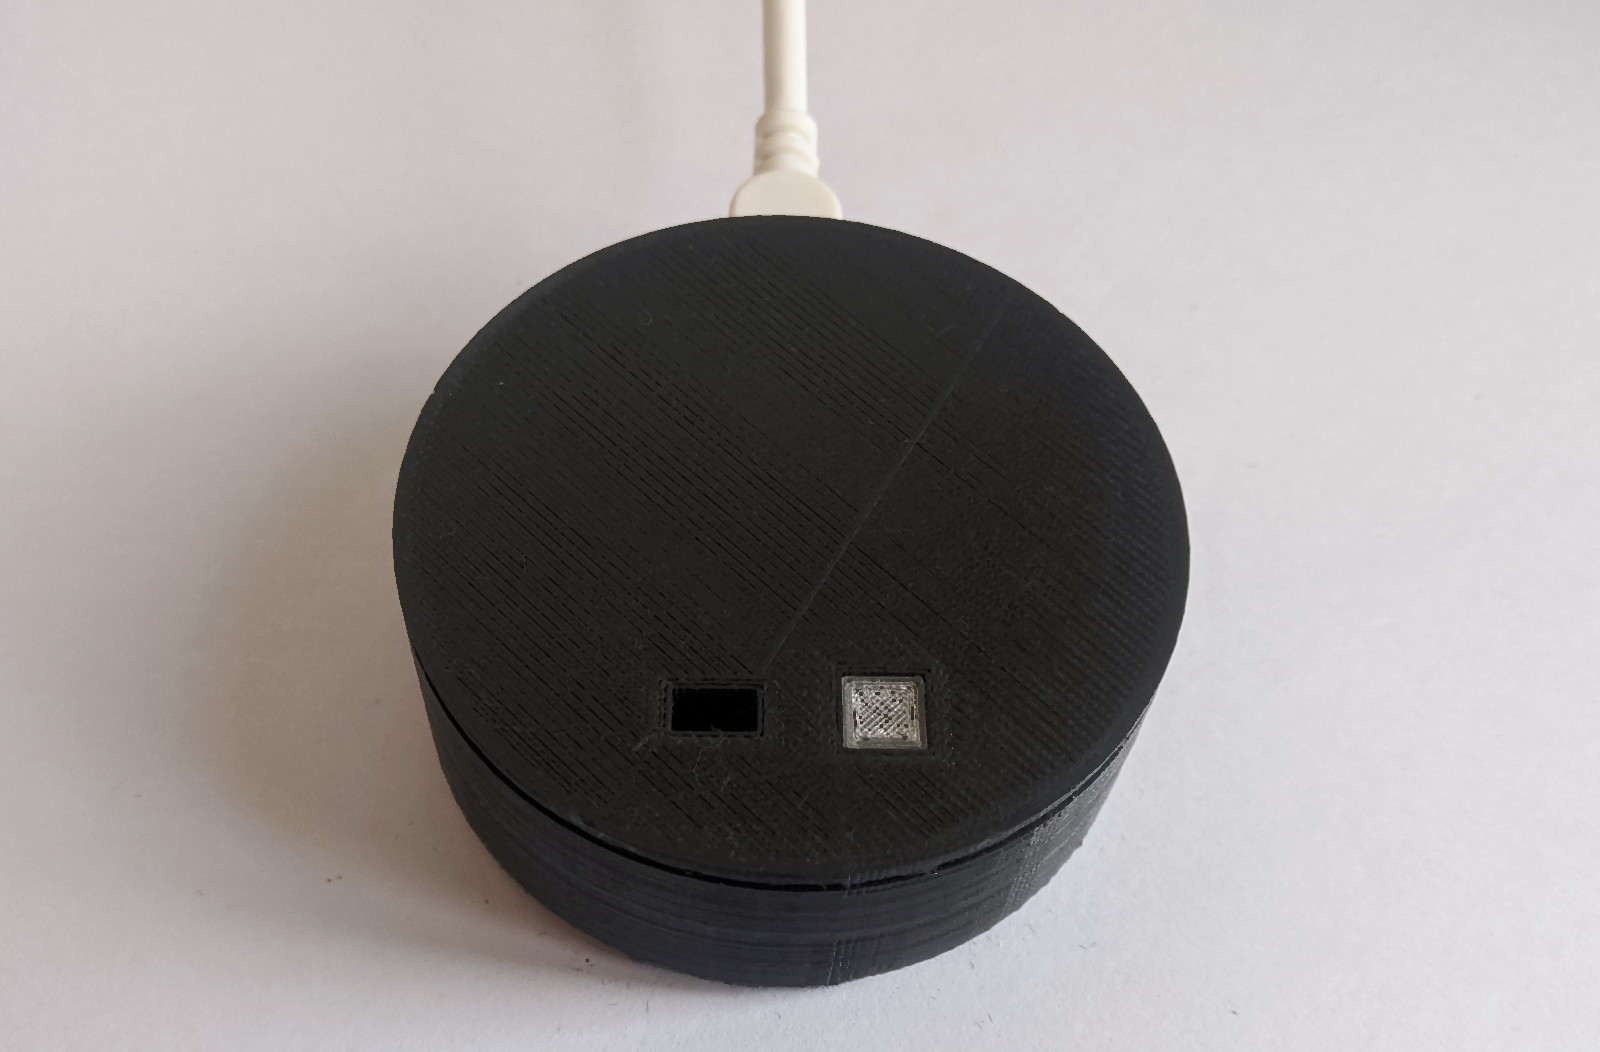
\includegraphics[scale=0.5]{Dispositivo_files/assembly_15.jpg}
	\end{figure}
	Una bella slide con una fotografia
\end{frame}

\begin{frame}
	\frametitle{La slide con la tabella}
	\begin{table}
		\centering
		\resizebox{\columnwidth}{!}{\begin{tabular}{|c|c|c|} 
			\hline
			\textbf{Configurazione (D14,D15)} & \textbf{Resistenza (k\si{\ohm})} & \textbf{Gain relativo}  \\ 
			\hline
			L,L & 24.334   & 1.000         \\ 
			\hline
			Z,L & 30.620   & 1.258         \\ 
			\hline
			L,Z & 51.123   & 2.101         \\ 
			\hline
			Z,Z & 337.847    & 13.883          \\
			\hline
		\end{tabular}}
	\end{table}
	Una bella slide con una tabella
\end{frame}

\section{Fine}
\begin{frame}
	\frametitle{Conclusioni}
	\lipsum[2]
\end{frame}

\end{document}
